\documentclass[12pt]{article}

\usepackage{graphicx}
\usepackage{float}
\usepackage{booktabs}
\usepackage{geometry}
\usepackage{hyperref}
\usepackage{listings}
\usepackage{xcolor}

\geometry{margin=1in}

% R code formatting
\lstset{
language=R,
basicstyle=\ttfamily\small,
keywordstyle=\color{blue},
stringstyle=\color{red},
commentstyle=\color{green!50!black},
breaklines=true,
frame=single
}

\title{NFL Play Calling Optimization}
\author{Karissa Merillat}
\date{\today}

\begin{document}

\maketitle

\begin{abstract}

This project examines play-calling tendencies in the NFL using play-by-play data and Expected Points Added (EPA). The goal is to evaluate how effectively teams choose between running and passing in different game situations. Using the \texttt{nflfastR} dataset, plays were broken down by down, distance, and field position to compare the impact of each play type. By analyzing the expected value of run versus pass plays, this study highlights where teams align with — or drift away from — data-driven, optimal decision-making.

\end{abstract}

\section{Introduction}

Play calling is one of the most important strategic decisions in football. Coaches must constantly decide whether to run or pass the ball based on game context such as down, distance, field position, and score differential.

Modern sports analytics has introduced quantitative tools that allow analysts to evaluate these decisions more objectively. One of the most widely used metrics in football analytics is Expected Points Added (EPA), which measures the change in expected points resulting from a play.

The goal of this project is to evaluate whether NFL teams make optimal play-calling decisions by comparing the average EPA of run and pass plays in different situations. By analyzing play-by-play data, we can identify situations where teams might benefit from adjusting their play-calling tendencies.

\section{Data Collection}

The play-by-play dataset was obtained using the \texttt{nflfastR} package in R, which provides detailed data for every NFL play. This dataset includes variables such as down, yards to go, field position, play type, score differential, and Expected Points Added.

\subsection{Loading the Data}

\begin{lstlisting}
library(nflfastR)
library(tidyverse)
library(arrow)

pbp <- load_pbp(2023)

glimpse(pbp)
\end{lstlisting}

The dataset contains detailed information for every play during the 2023 NFL season.

\section{Data Preparation}

Before performing the analysis, the dataset was filtered and transformed to focus on meaningful play-calling decisions.

\subsection{Filtering Run and Pass Plays}

Only plays where teams chose to run or pass were included.

\begin{lstlisting}
plays <- pbp %>%
  filter(play_type %in% c("run", "pass"))
\end{lstlisting}

\subsection{Creating Distance Categories}

Distance to first down was categorized into short, medium, and long situations.

\begin{lstlisting}
plays <- plays %>%
  mutate(distance_cat = case_when(
    ydstogo <= 3 ~ "short",
    ydstogo <= 7 ~ "medium",
    TRUE ~ "long"
  ))
\end{lstlisting}

\subsection{Creating Field Position Categories}

Field position was divided into several zones to better capture contextual game situations.

\begin{lstlisting}
plays <- plays %>%
  mutate(field_zone = case_when(
    yardline_100 >= 60 ~ "own_territory",
    yardline_100 >= 40 ~ "midfield",
    yardline_100 <= 20 ~ "red_zone",
    TRUE ~ "opponent_territory"
  ))
\end{lstlisting}

\subsection{Removing Fourth Down Plays}

Fourth down decisions involve different strategic considerations, so only downs 1 through 3 were analyzed.

\begin{lstlisting}
plays <- plays %>%
  filter(down %in% c(1,2,3))
\end{lstlisting}

\subsection{Creating Game Situations}

Game situations were defined using down, distance category, and field zone.

\begin{lstlisting}
plays <- plays %>%
  mutate(situation = paste(down, distance_cat, field_zone))
\end{lstlisting}

\subsection{Removing Garbage Time}

Plays with extreme score differences were removed to avoid distortions caused by late-game situations.

\begin{lstlisting}
plays <- plays %>%
  filter(abs(score_differential) <= 16)
\end{lstlisting}

\section{Methodology}

To evaluate play-calling efficiency, the average Expected Points Added (EPA) was calculated separately for run and pass plays in each situation.

\subsection{Calculating Average EPA}

\begin{lstlisting}
epa_summary <- plays %>%
  group_by(situation, play_type) %>%
  summarize(
    avg_epa = mean(epa, na.rm = TRUE),
    plays = n()
  ) %>%
  arrange(situation)
\end{lstlisting}

\subsection{Comparing Run and Pass Efficiency}

The dataset was reshaped so that run and pass EPA values could be compared directly.

\begin{lstlisting}
epa_compare <- epa_summary %>%
  select(situation, play_type, avg_epa) %>%
  pivot_wider(
    names_from = play_type,
    values_from = avg_epa
  )
\end{lstlisting}

\subsection{Pass Advantage Metric}

A metric called \textit{Pass Advantage} was created to measure the difference in expected value between passing and running.

\[
Pass\ Advantage = EPA_{pass} - EPA_{run}
\]

\begin{lstlisting}
epa_compare <- epa_compare %>%
  mutate(pass_advantage = pass - run)
\end{lstlisting}

Positive values indicate situations where passing produces higher expected value.

\section{Play Calling Behavior}

To evaluate real coaching decisions, the frequency of run and pass plays was calculated for each situation.

\begin{lstlisting}
play_call_rates <- plays %>%
  group_by(situation, play_type) %>%
  summarize(plays = n(), .groups = "drop") %>%
  group_by(situation) %>%
  mutate(
    total_plays = sum(plays),
    play_pct = plays / total_plays
  )
\end{lstlisting}

These rates were then merged with the EPA results.

\begin{lstlisting}
analysis_table <- play_call_compare %>%
  left_join(epa_compare, by = "situation")
\end{lstlisting}

\section{Results}

\subsection{Pass Advantage Visualization}

\begin{figure}[H]
\centering
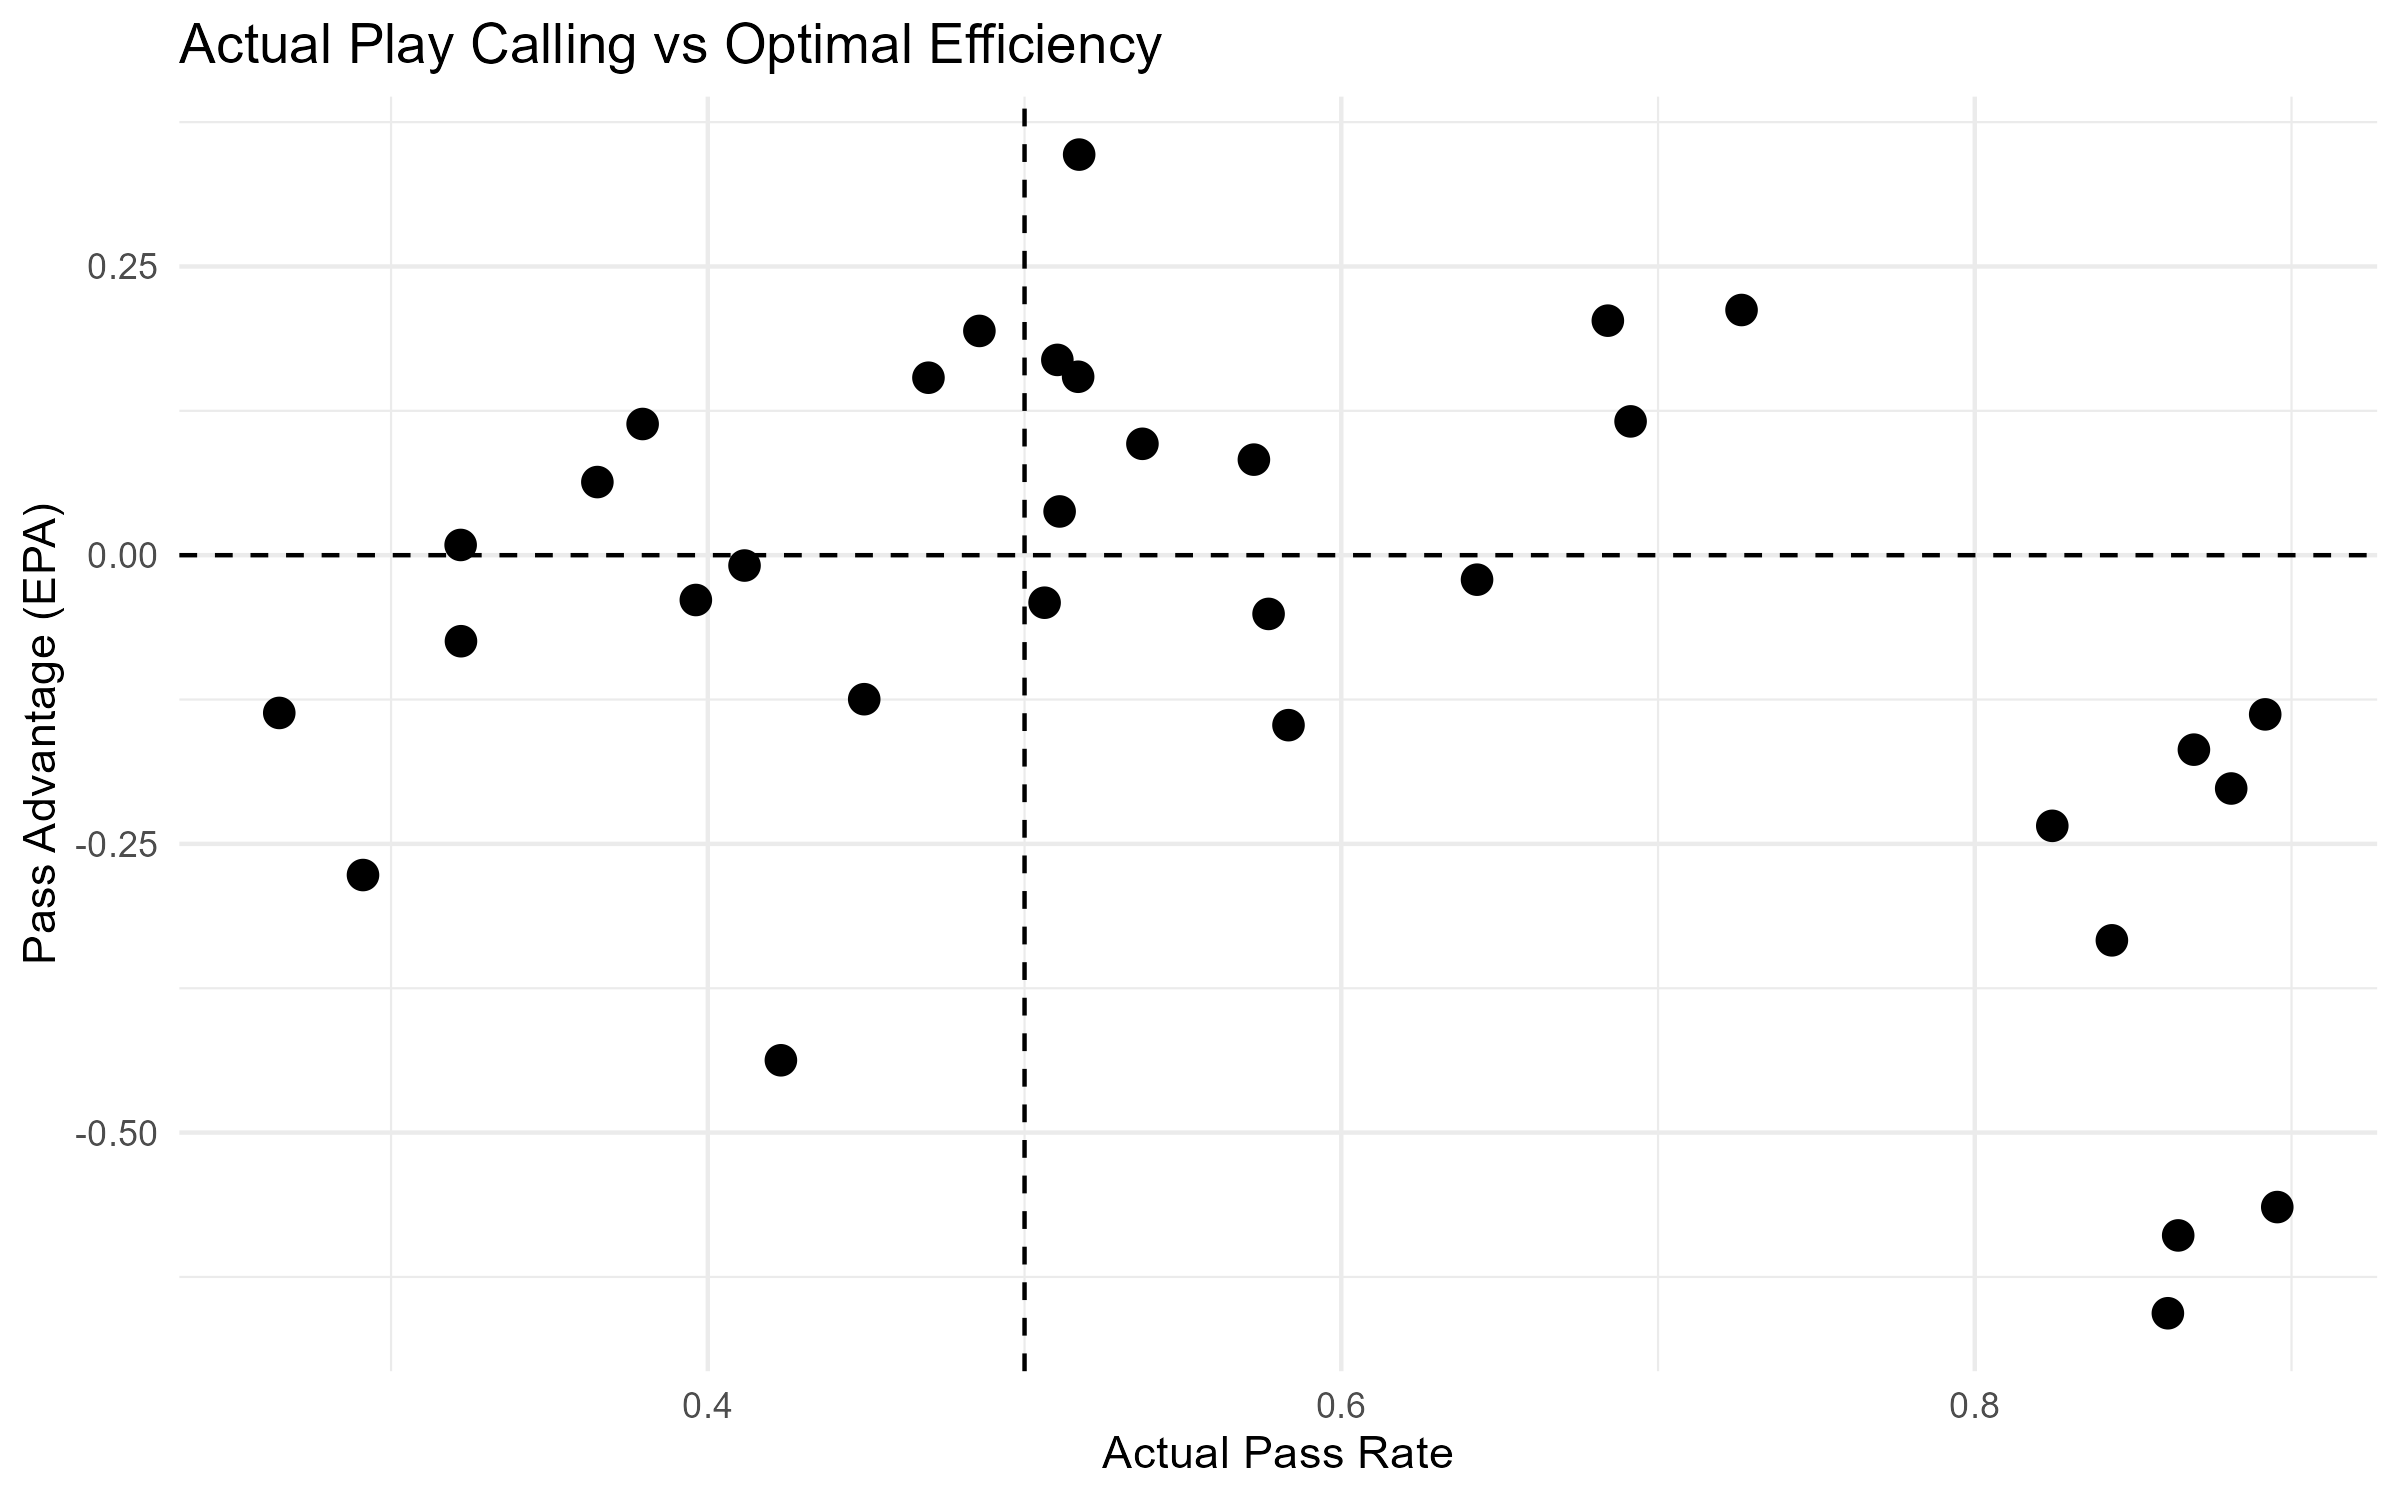
\includegraphics[width=0.85\textwidth]{pass_advantage_chart.png}
\caption{Pass Advantage (EPA Difference) by Game Situation}
\end{figure}

The figure above displays the difference in Expected Points Added (EPA) between passing and running for each game situation. Positive values indicate that passing produces a higher expected value than running, while negative values indicate that running is more efficient.

Several situations show a clear advantage for passing, particularly in longer yardage scenarios. Despite this, teams do not always adjust their play-calling behavior accordingly. This suggests that there may be inefficiencies in how teams balance run and pass decisions based on game context.

\subsection{Horizontal Pass Advantage Chart}

\begin{figure}[H]
\centering
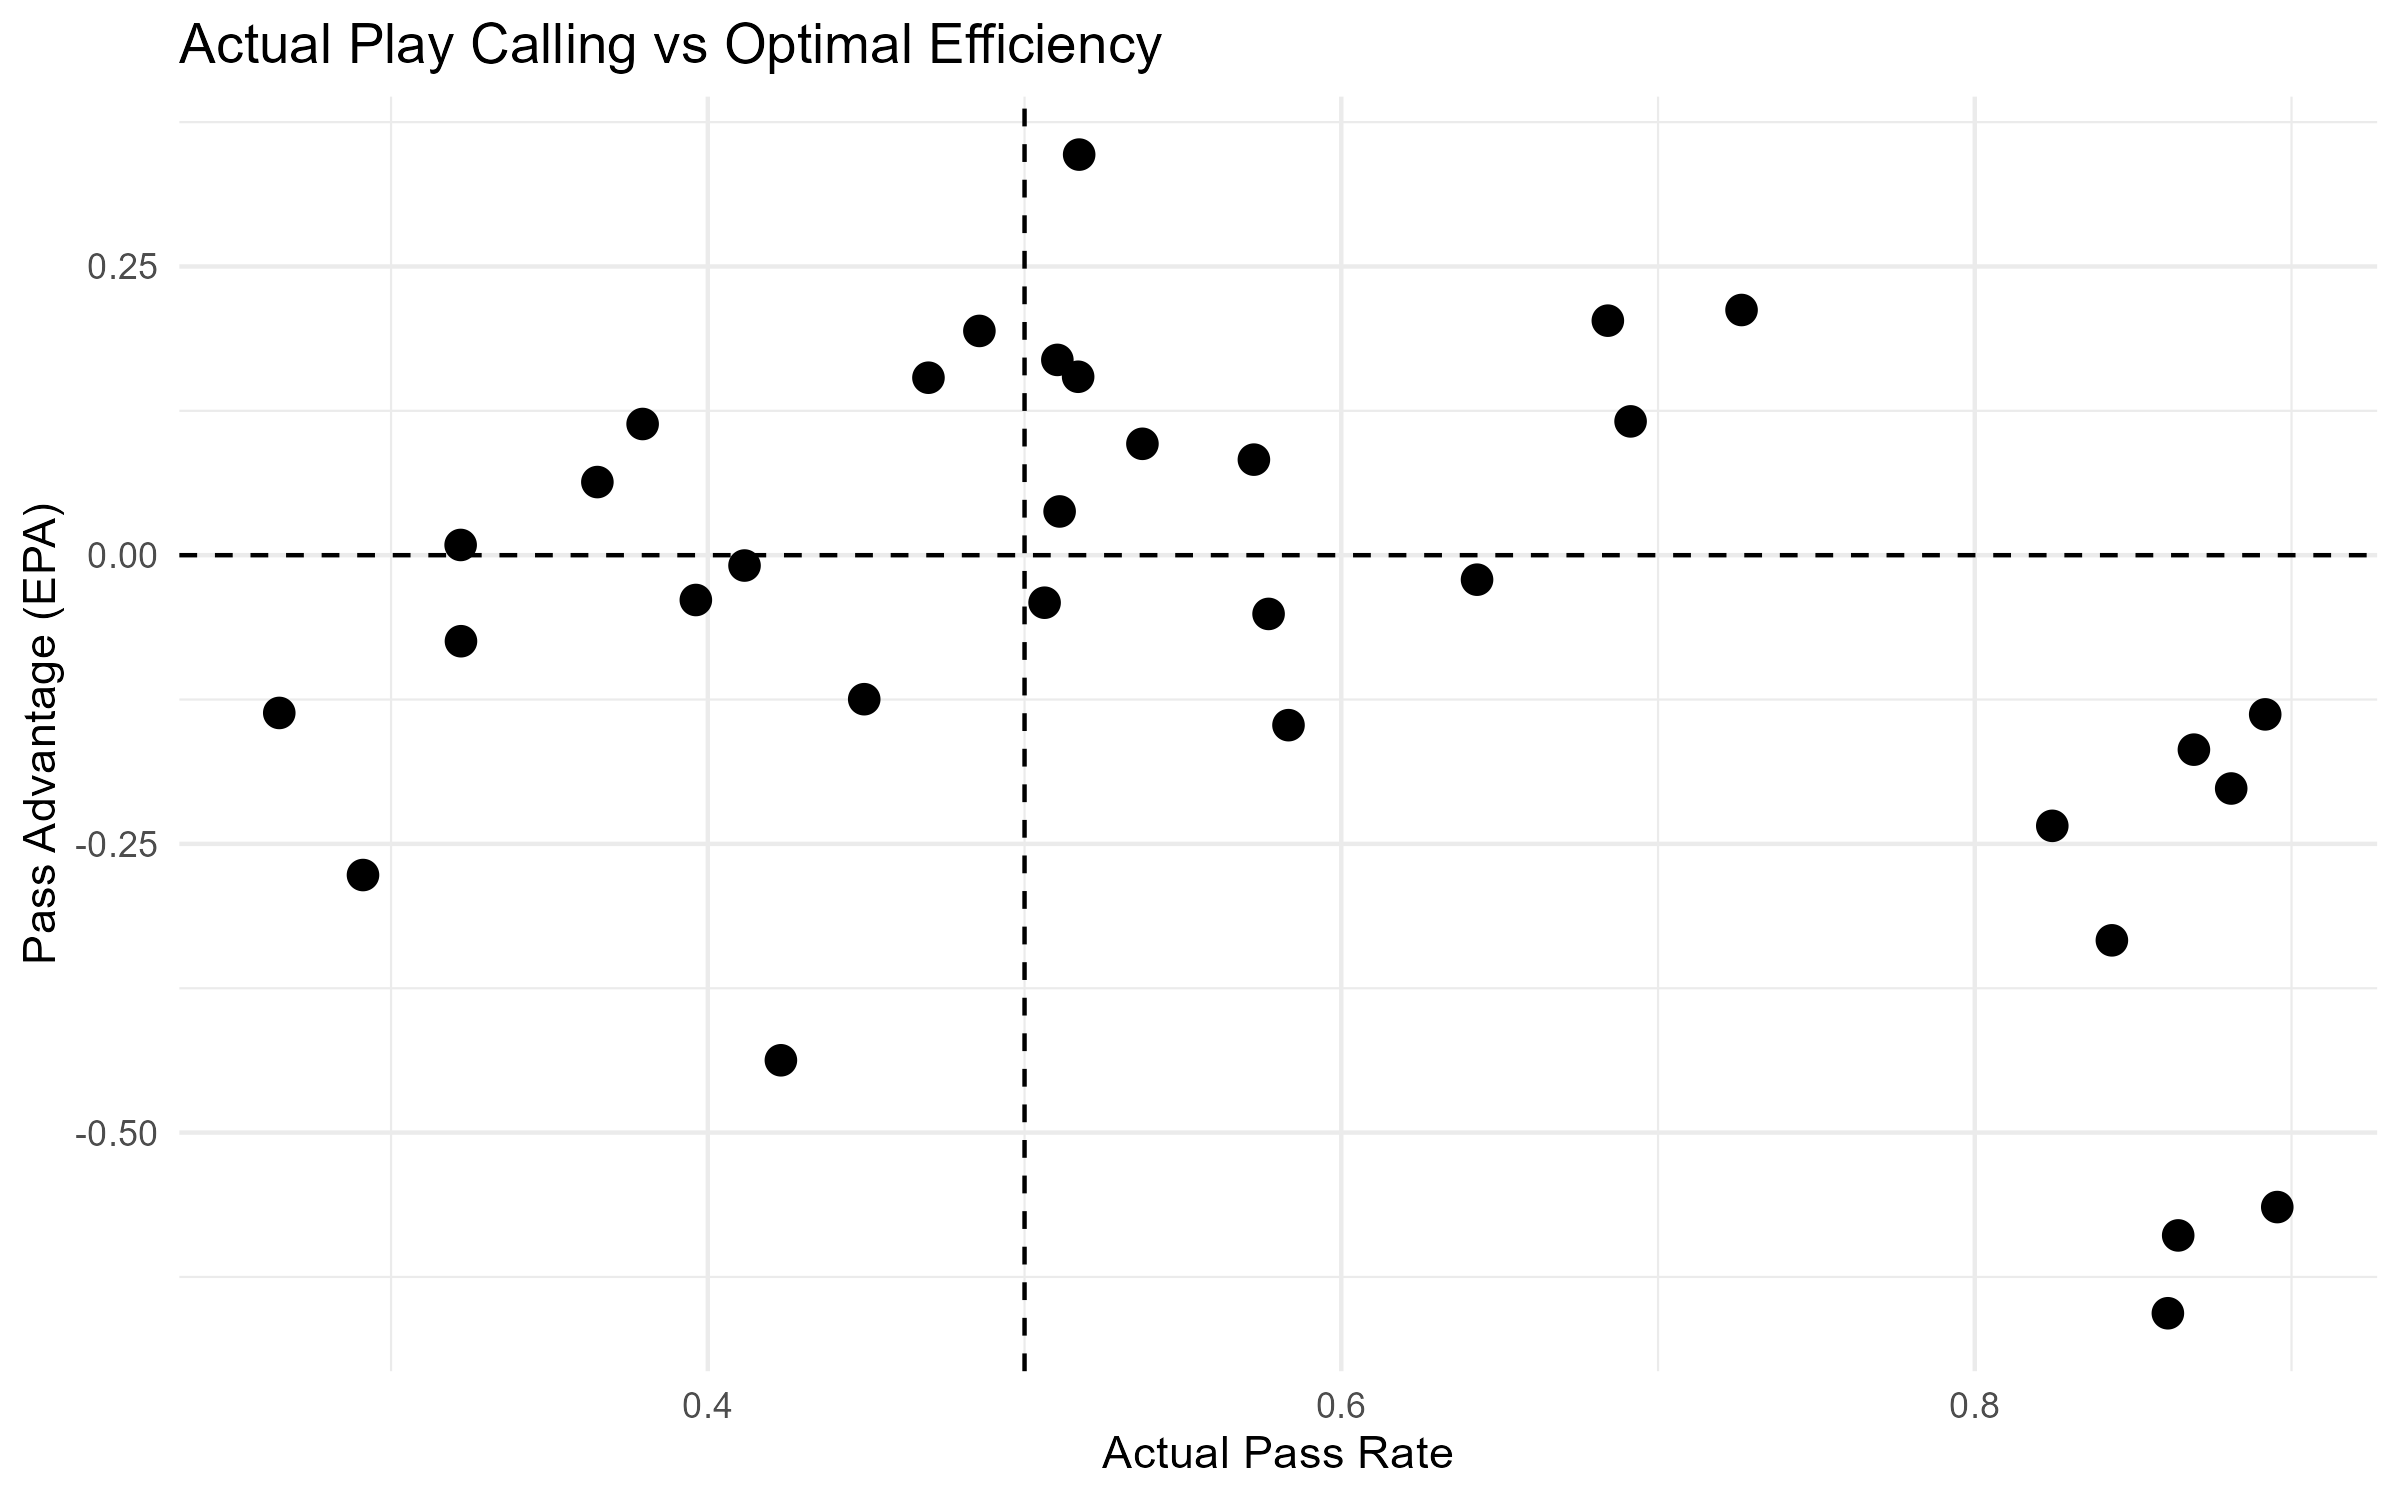
\includegraphics[width=0.85\textwidth]{pass_advantage_flip.png}
\caption{Pass Advantage by Situation}
\end{figure}

This horizontal bar chart presents the same pass advantage data in a more readable format, allowing for easier comparison across situations. The visualization highlights which specific combinations of down, distance, and field position favor passing or running.

Situations with the largest positive values represent the greatest opportunities for increased passing efficiency, while negative values indicate scenarios where running is the better option. This chart helps clearly identify where strategic adjustments could yield the greatest improvement.

\subsection{Actual Play Calling vs Optimal Strategy}

\begin{figure}[H]
\centering
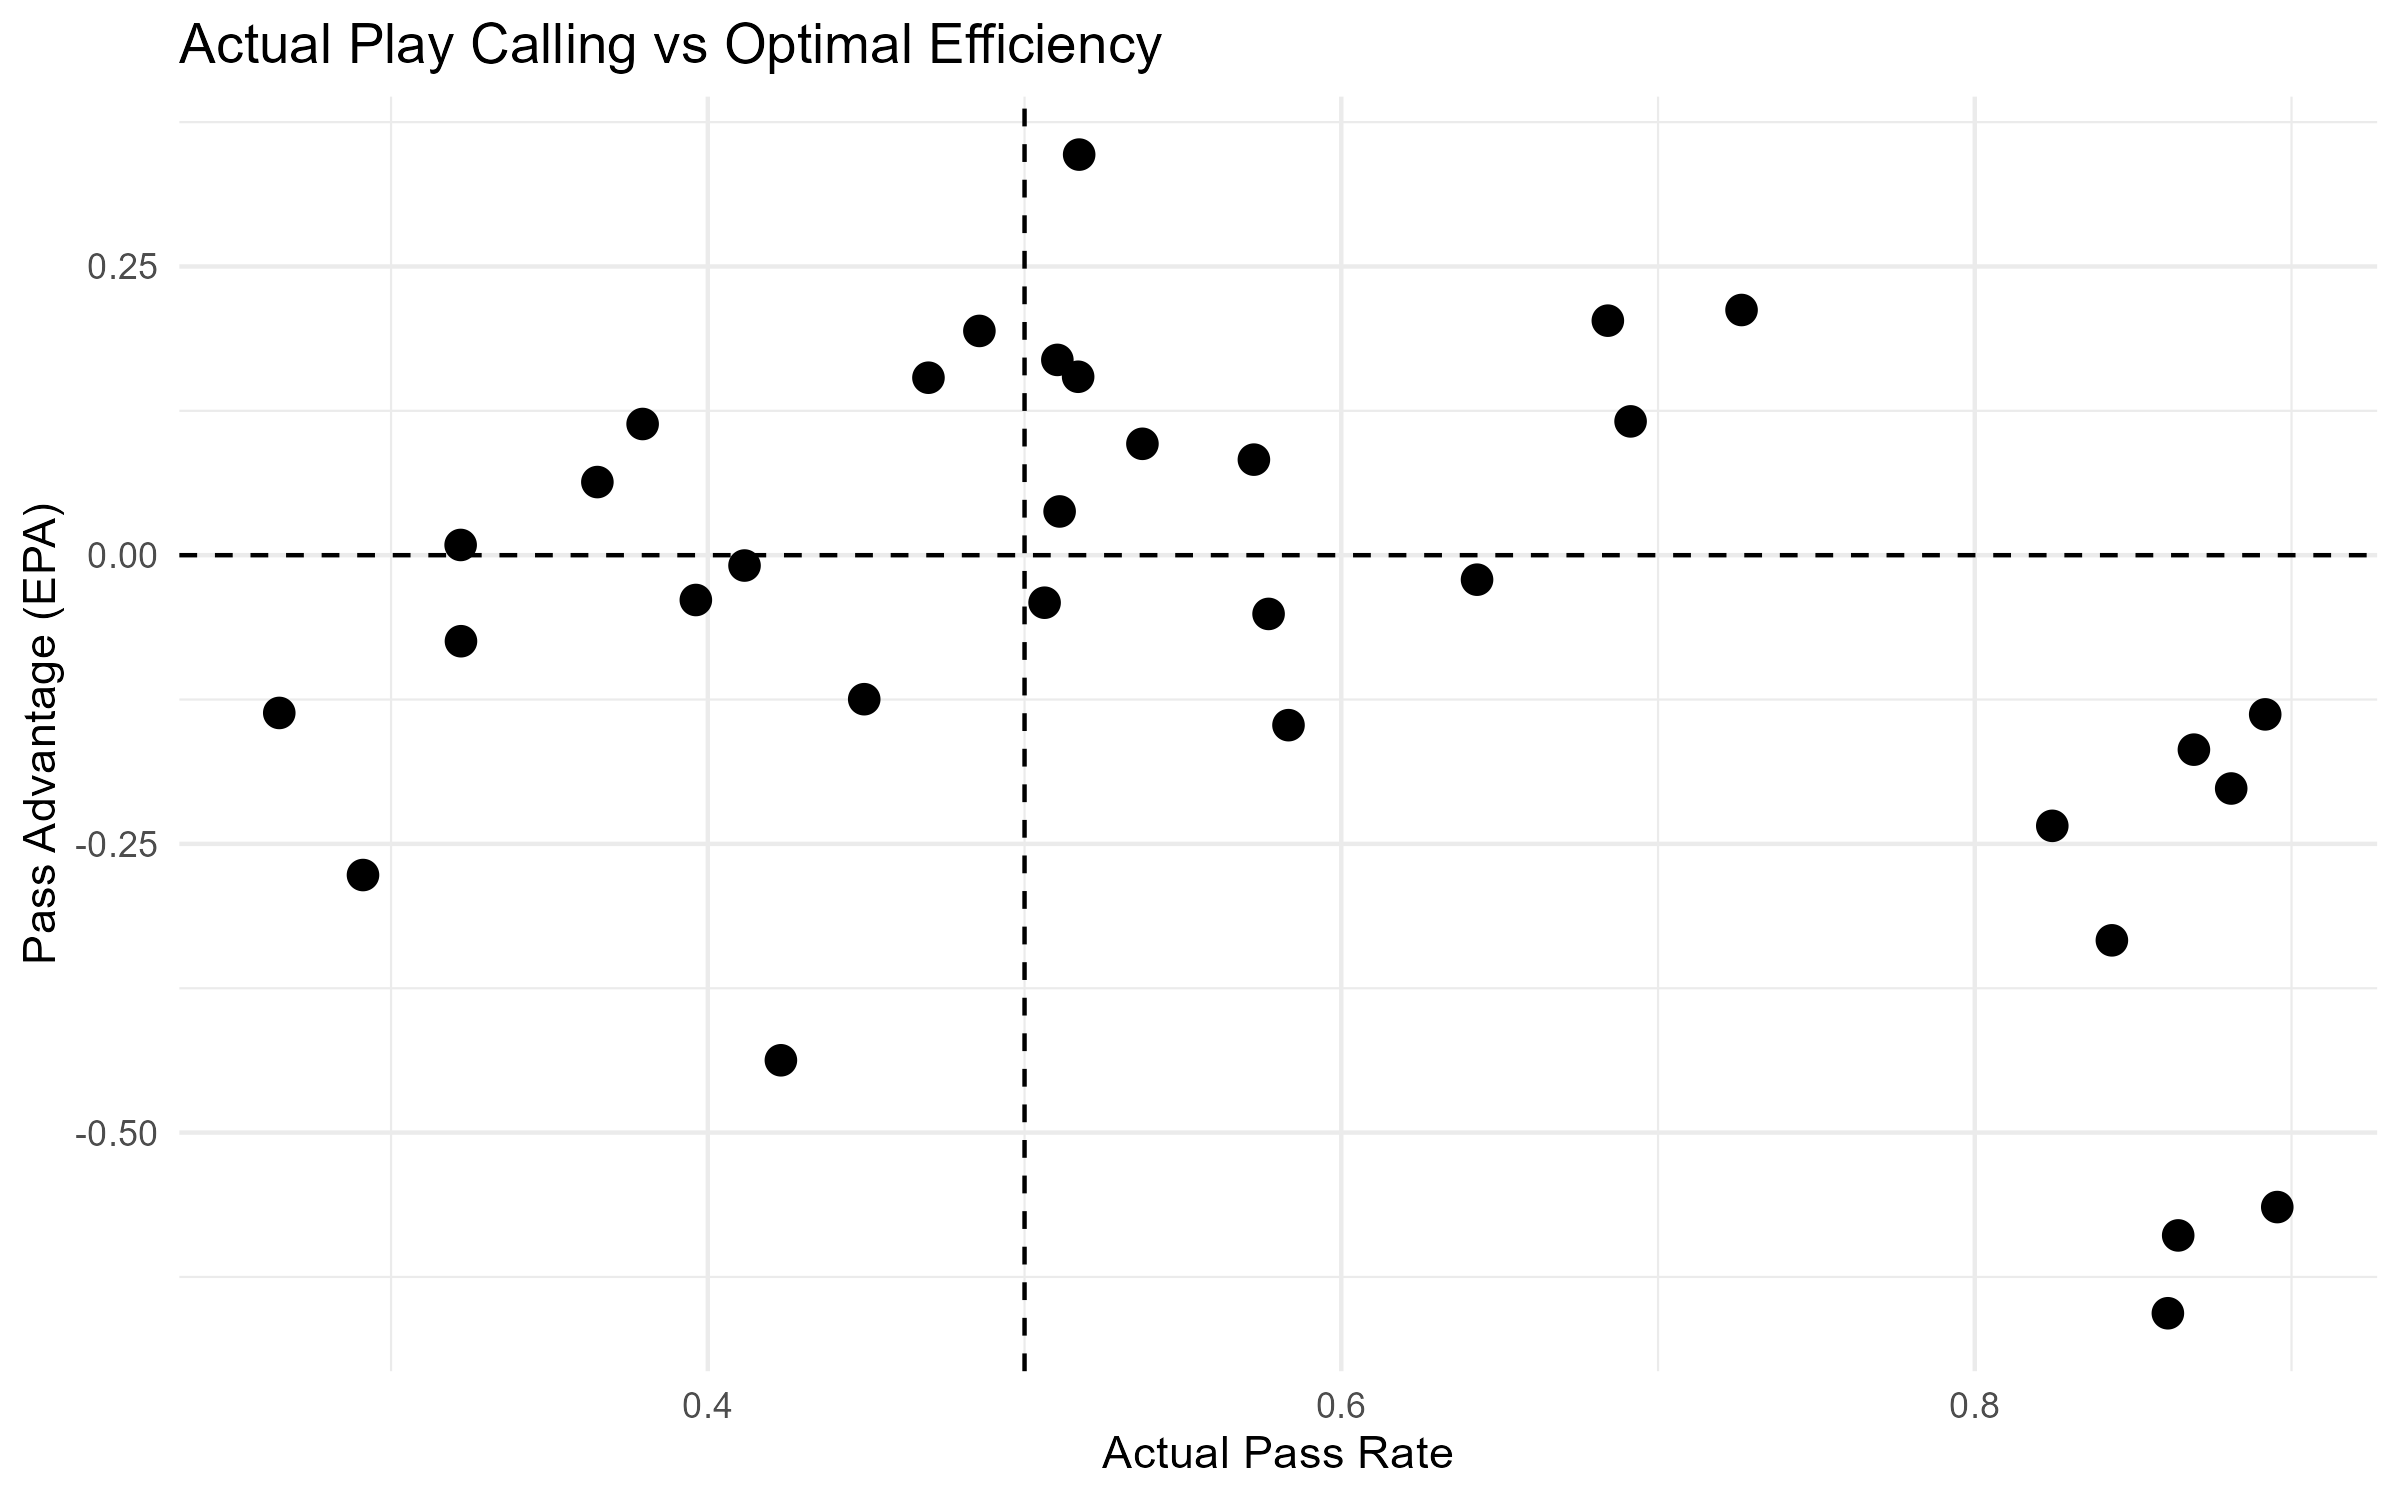
\includegraphics[width=0.85\textwidth]{play_calling_efficiency.png}
\caption{Actual Play Calling vs Optimal Efficiency}
\end{figure}

This scatter plot compares actual play-calling tendencies with the measured efficiency of passing versus running. The horizontal axis represents the actual pass rate used by teams, while the vertical axis represents the pass advantage in terms of EPA.

The dashed horizontal line at zero separates situations where passing is more efficient (above the line) from those where running is more efficient (below the line). The vertical dashed line represents a balanced play-calling approach.

Points located in the upper-left region of the graph indicate situations where passing is more effective, but teams still run frequently. These points highlight the most significant inefficiencies in play calling. Conversely, points in the lower-right region suggest situations where teams may pass more often than optimal.

Overall, this visualization provides a clear framework for evaluating whether coaching decisions align with analytically optimal strategies.

\subsection{Results Summary}

Together, the visualizations reveal meaningful differences between actual NFL play-calling tendencies and analytically optimal decisions. The pass advantage charts demonstrate that in several situations, particularly those involving longer yardage, passing generates a higher Expected Points Added than running in high-leverage situations. However, the play-calling frequency data shows that teams often continue to favor the run even when passing provides greater expected value.

The scatter plot further emphasizes these inefficiencies by identifying situations where teams underutilize passing despite its strategic advantage. These patterns suggest that NFL teams may rely on conservative tendencies rather than fully optimizing decisions based on expected outcomes.

Overall, the results indicate that while teams often make efficient decisions, there remain several game situations where data-driven adjustments to play calling could improve offensive efficiency.

\section{Discussion}

The results suggest that NFL teams do not always follow analytically optimal strategies when selecting plays. In several situations, passing produces a higher Expected Points Added than running, yet teams continue to favor running plays.

This behavior may reflect coaching preferences, perceived risk, or strategic considerations not captured by EPA alone.

Future research could expand this analysis to multiple seasons or incorporate win probability models to better capture the strategic complexity of football decision-making.


\section{Conclusion}

This study analyzed NFL play-calling decisions using Expected Points Added to compare the efficiency of run and pass plays. By grouping plays into specific game situations, it was possible to identify patterns in play-calling behavior and evaluate whether teams are making optimal decisions.

The findings illustrate how data-driven analysis can provide insights into coaching strategy and highlight opportunities for improved decision-making in professional football.

\end{document}

\begin{figure}
    \centering
    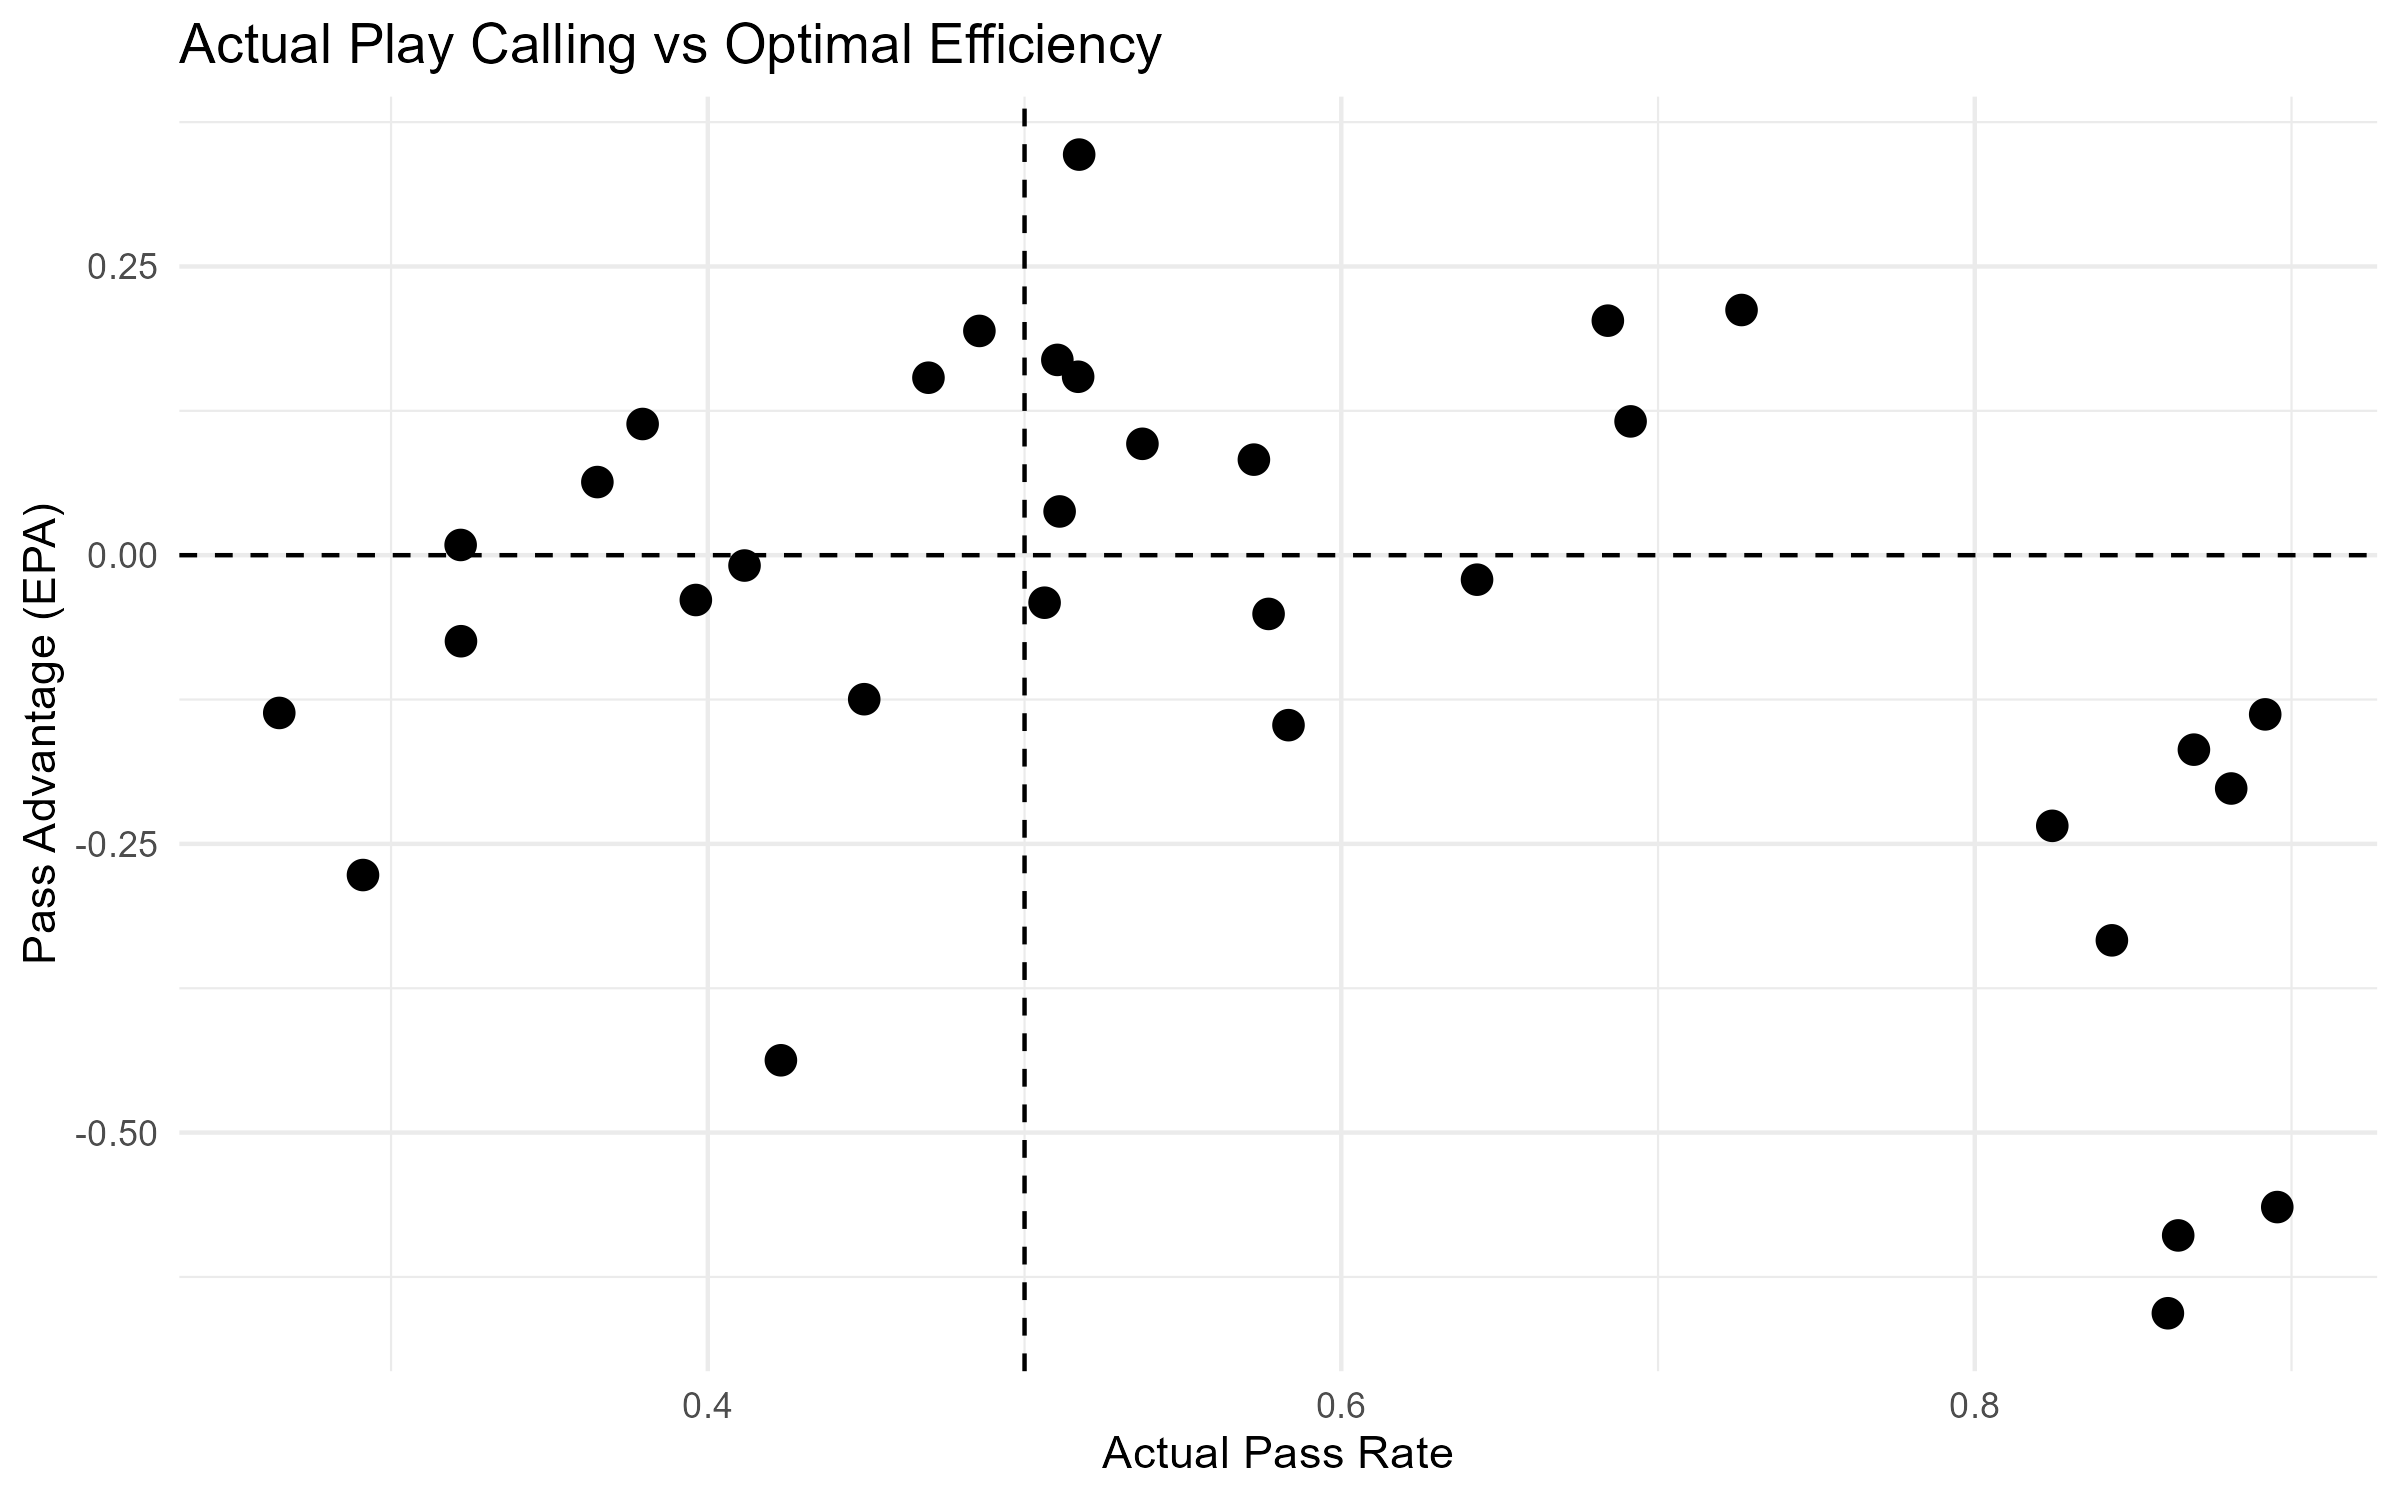
\includegraphics[width=0.5\linewidth]{play_calling_efficiency.png}
    \caption{Enter Caption}
    \label{fig:placeholder}
\end{figure}
\begin{figure}
    \centering
    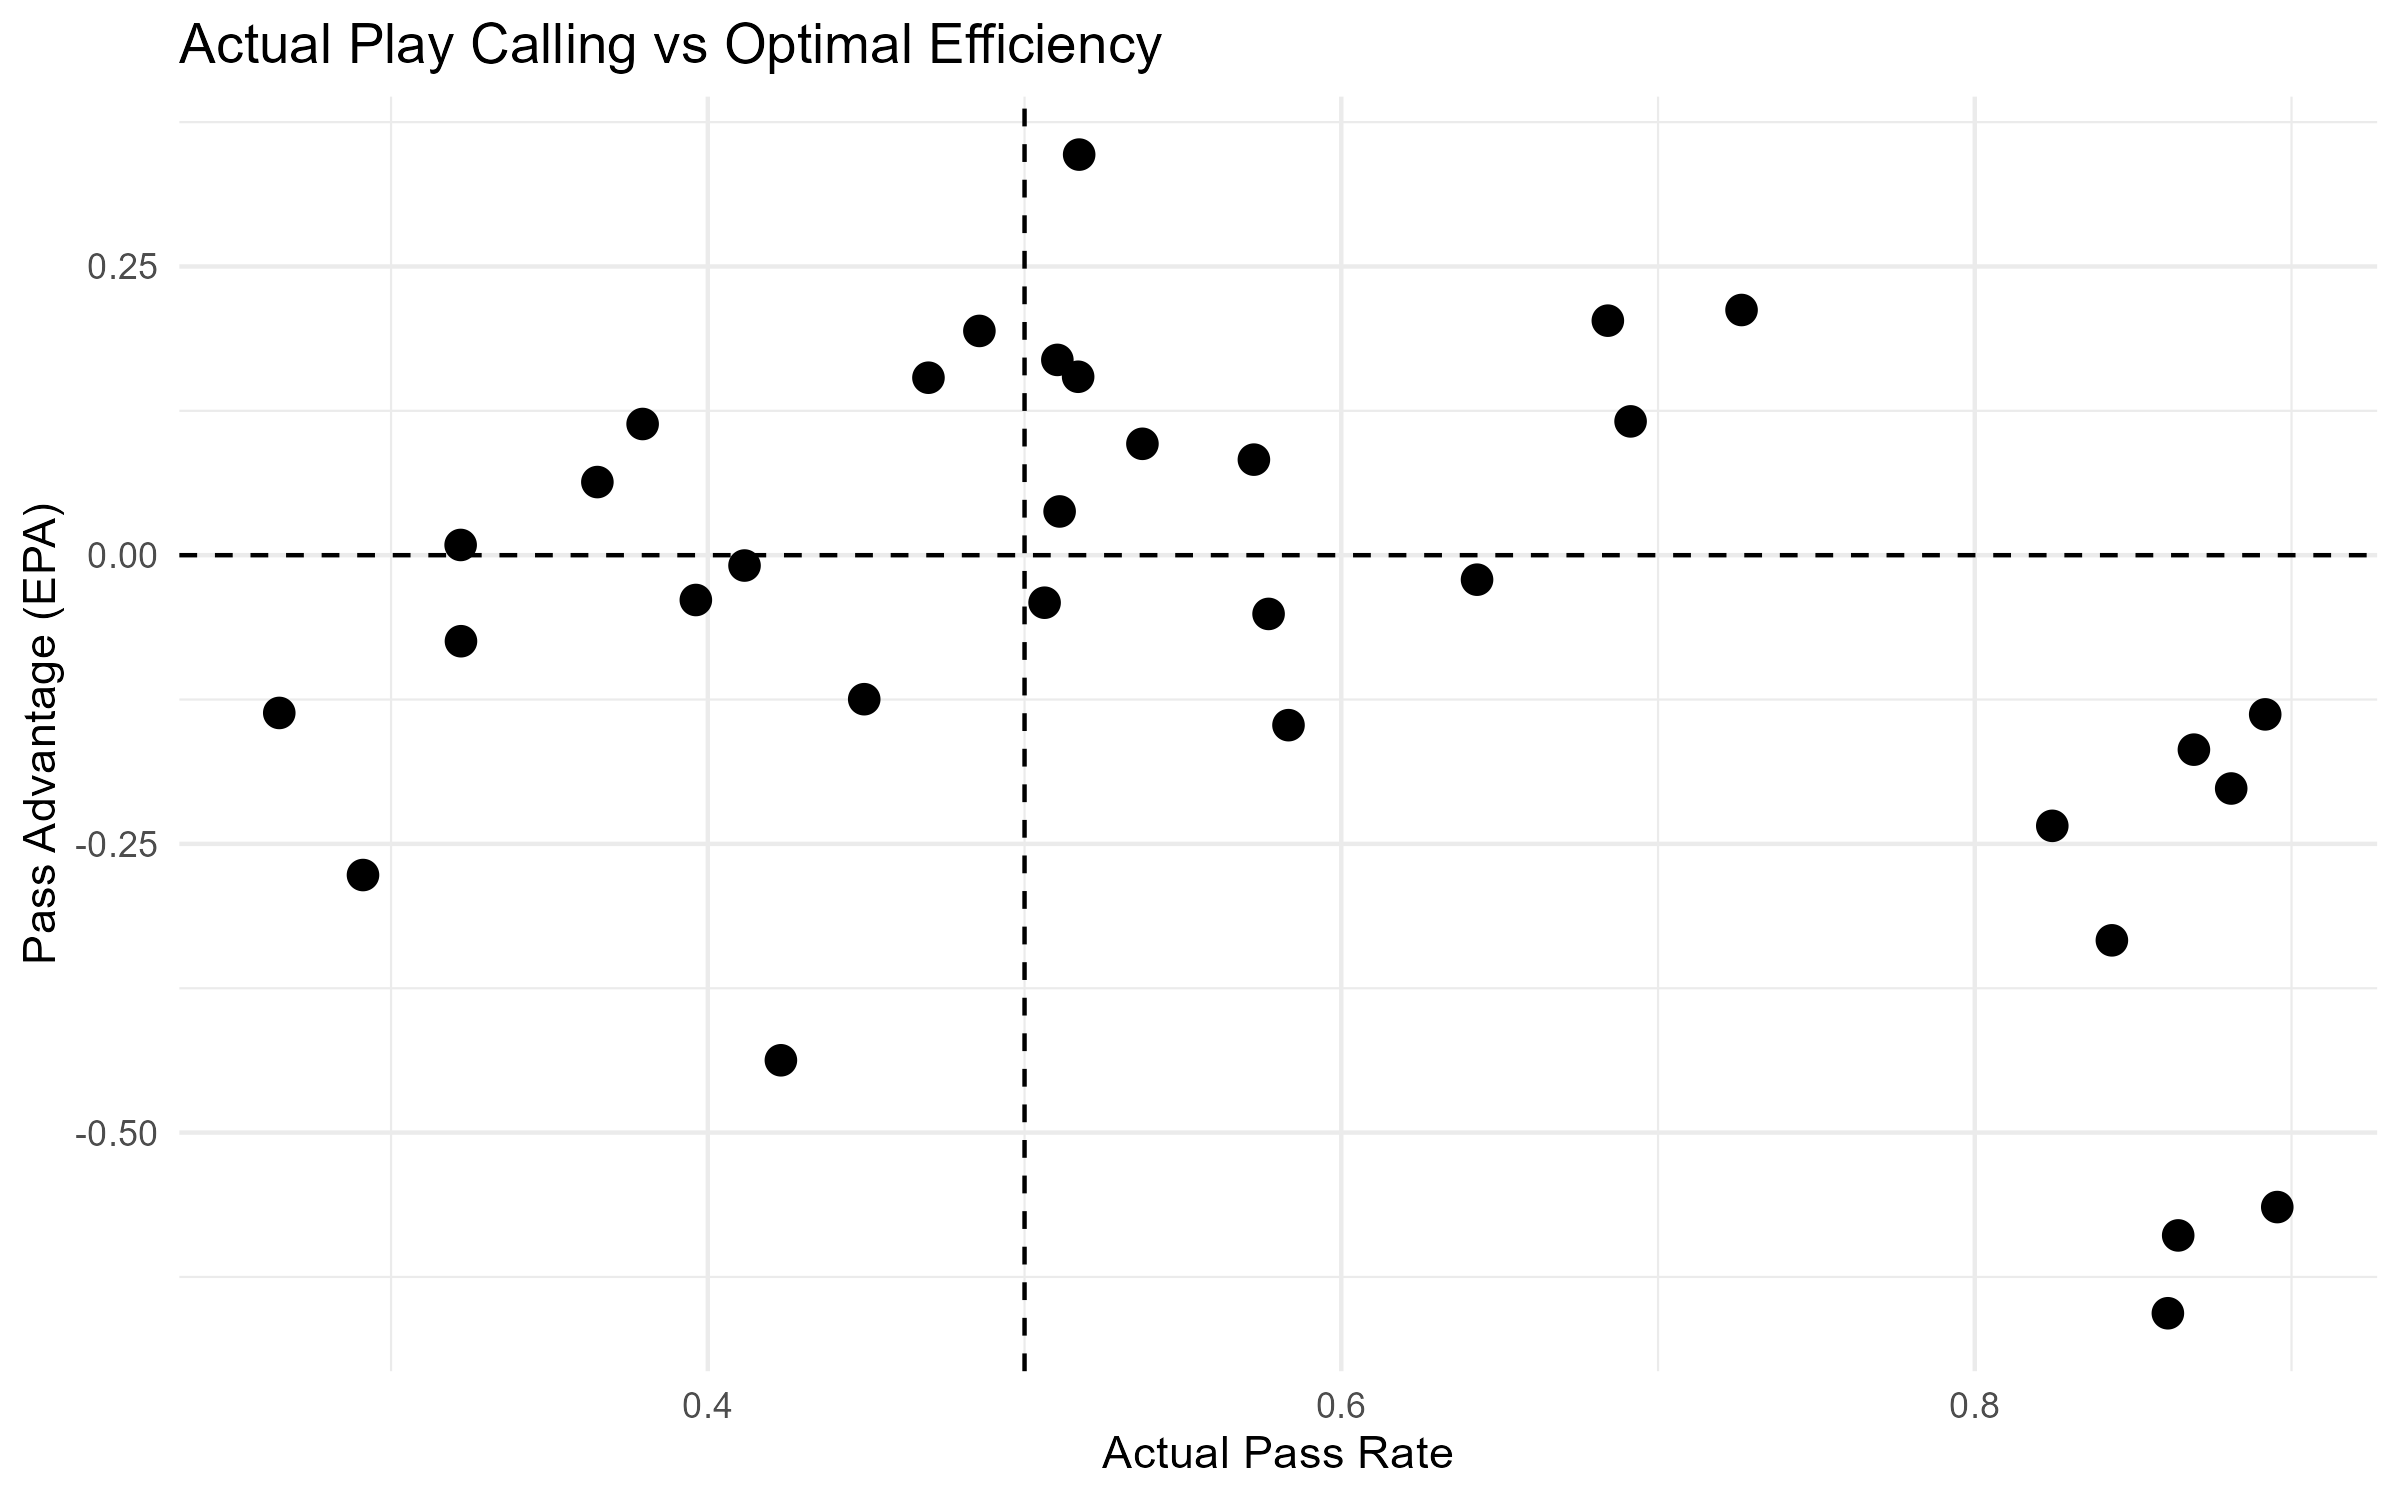
\includegraphics[width=0.5\linewidth]{pass_advantage_flip.png}
    \caption{Enter Caption}
    \label{fig:placeholder}
\end{figure}
\begin{figure}
    \centering
    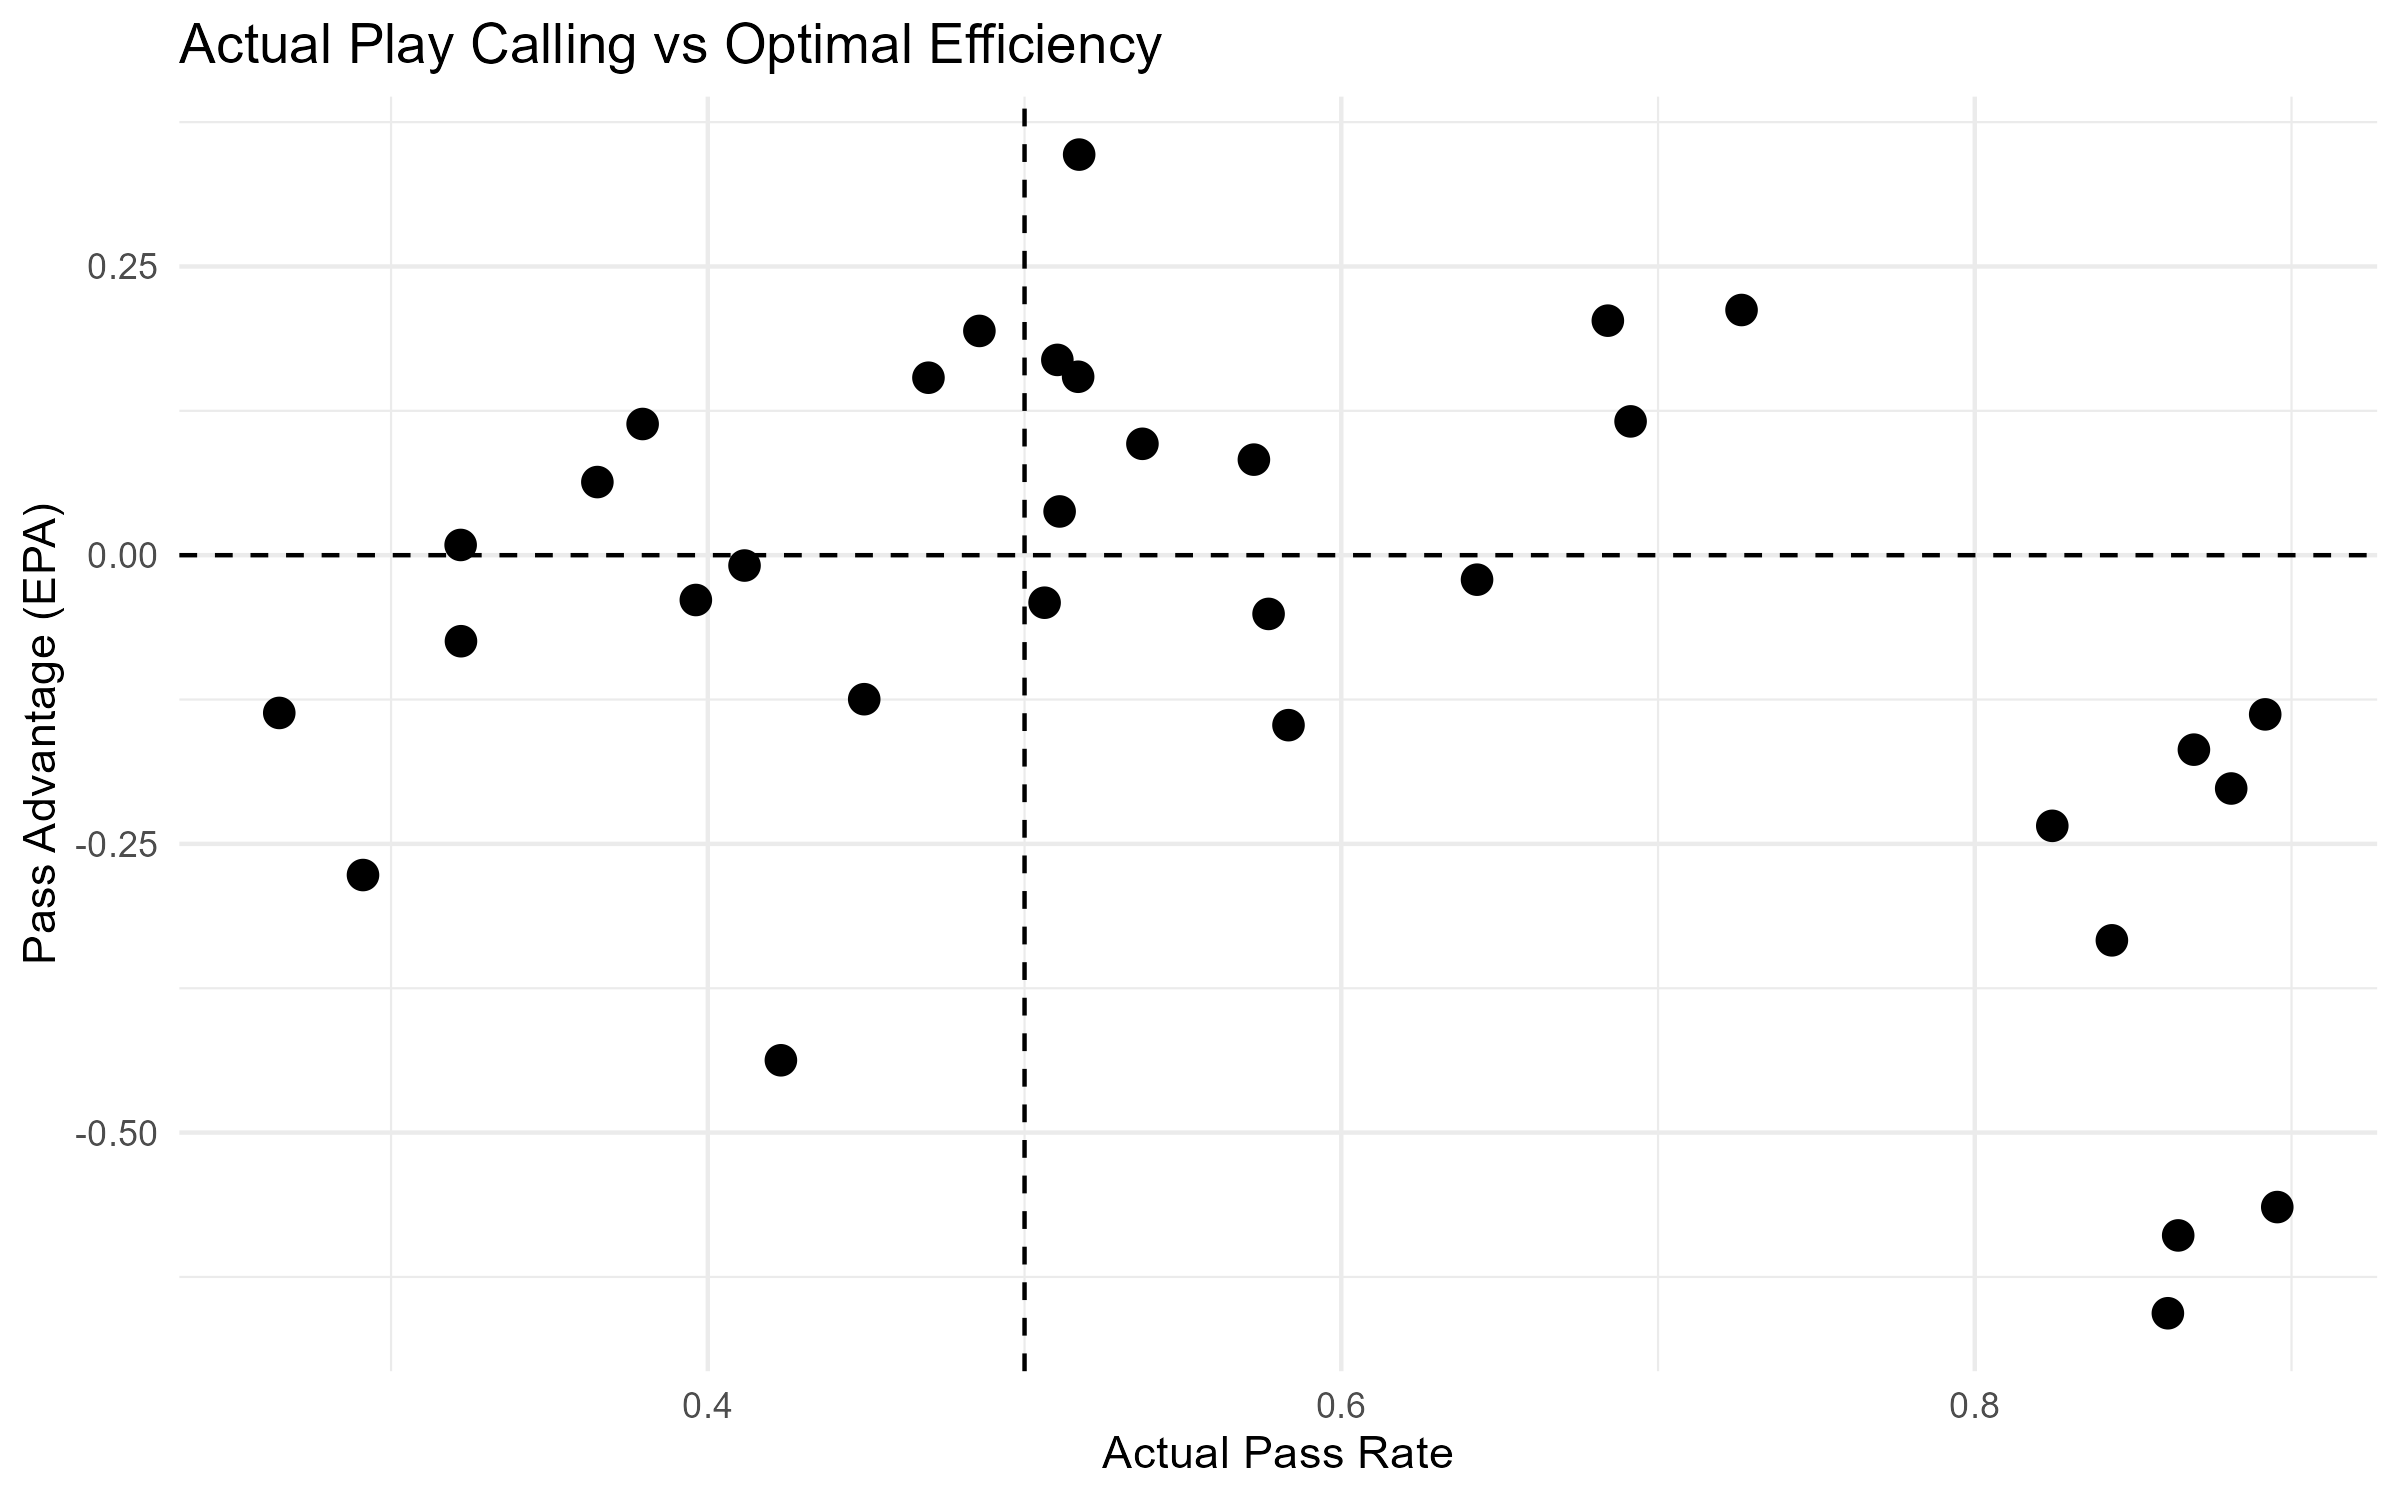
\includegraphics[width=0.5\linewidth]{pass_advantage_chart.png}
    \caption{Enter Caption}
    \label{fig:placeholder}
\end{figure}
